\usepackage{amsthm}

\newtheorem{theorem}{Theorem}[chapter]
\newtheorem{lemma}           [theorem] {Lemma}   
\newtheorem{folg}           [theorem] {Folgerung}   

\newtheorem{frage}       [theorem] {Frage}   
\newtheorem{question}       [theorem] {Question}   
\newtheorem{aufgabe}       [theorem] {Aufgabe}   
\newtheorem{exercise}       [theorem] {Exercise}  

\newtheorem{proposition}     [theorem] {Proposition}  
\newtheorem{satz}     [theorem] {Satz}  
\newtheorem{fact}{Fact}
\newtheorem{definition}      [theorem] {Definition} 

\theoremstyle{definition} 
\newtheorem{bemerkung}     [theorem] {Bemerkung}  
\newtheorem{beispiel}       [theorem] {Beispiel}  
\newtheorem{example}       [theorem] {Example}  
\newtheorem*{example*} {Example}  
\newtheorem{notation}       [theorem] {Notation}  
\newtheorem*{Faust}[theorem]{Rule of Thumb}
\newtheorem*{Boxx}[theorem]{Concept}

%\section{Differentiability and Derivatives}
To motivate the problem, consider the functions $f,g:\mathbb{R}\to\mathbb{R}$ with $f(x)=x^2$ and $g(x)=|x|$.

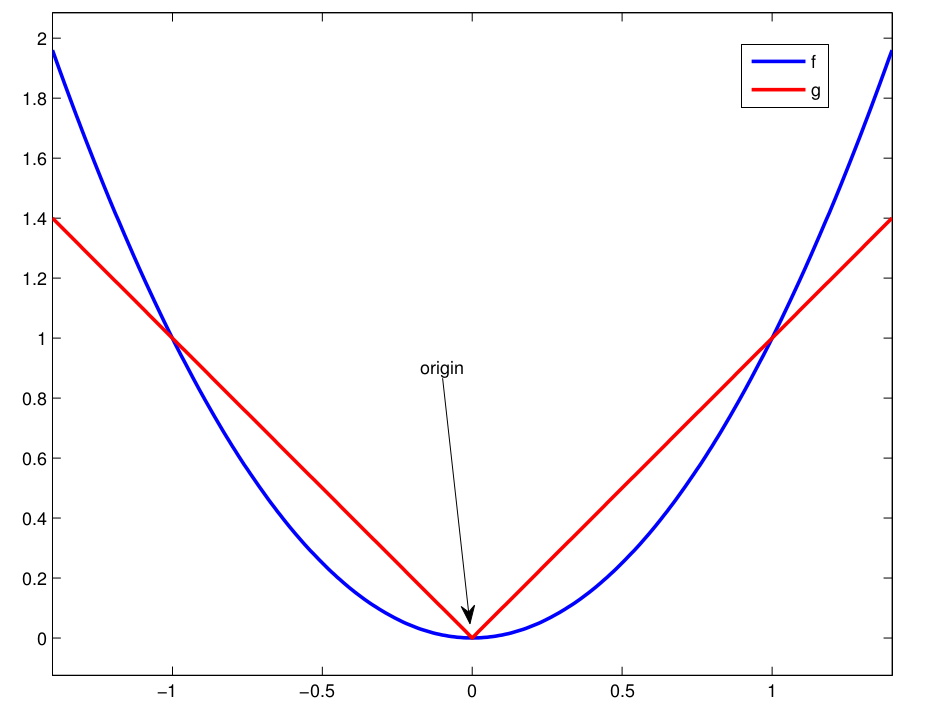
\includegraphics{./dom.png}

As we already know, both these functions are continuous. Let us now focus on the qualitative behavior of the functions at the origin.
\renewcommand{\arraystretch}{1.5}
\begin{table}[h!]\begin{center}
\begin{tabular}{|l|l|}
\hline $f$&$g$\\
\hline\hline&\\[-0.7cm]
smooth& sharp bend\\\hline
there is a unique tangent& no unique tangent\\\hline
\end{tabular}~\\~\\\caption{Qualitative behavior of $f$ and $g$ at the origin}\label{tab:ewcf}\end{center}
\end{table}
\renewcommand{\arraystretch}{1}\newpage
A~straight line $y(t)$ going through the points $(x_0,f(x_0))$ and $(x,f(x))$ is called
\emph{secant}~\footnote{from the Latin word {\em secare} = ``to cut''}
 of $f$ through these points. It is given by
\[y(t)=f(x_0)+\frac{f(x_0)-f(x)}{x_0-x}(t-x_0) .\]
In particular, the \emph{slope} of $y$ is the \emph{difference quotient}
\[\frac{f(x_0)-f(x)}{x_0-x}=\frac{f(x)-f(x_0)}{x-x_0}.\]

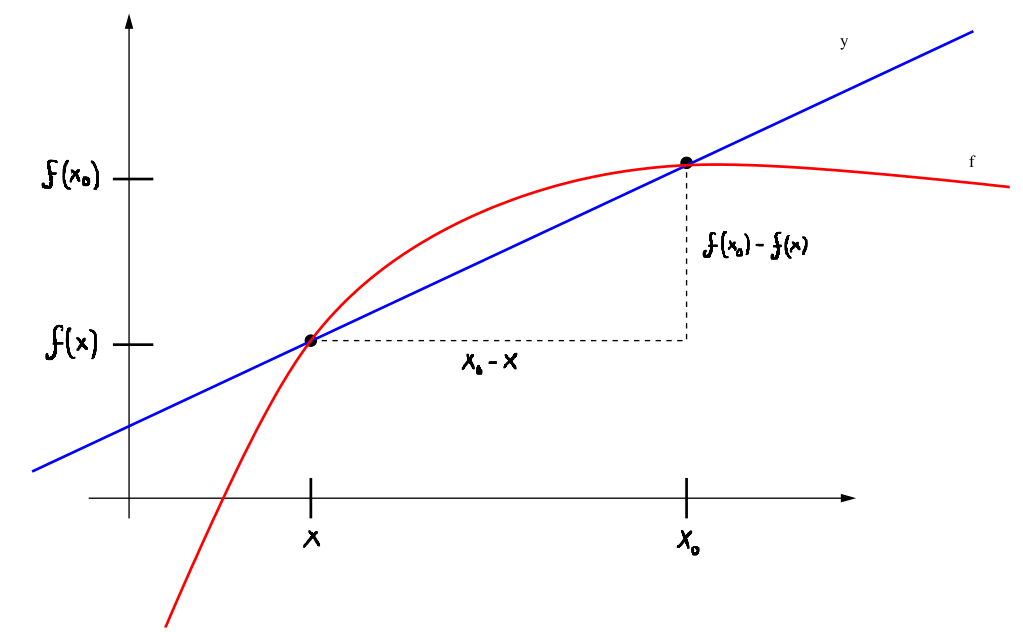
\includegraphics{./sec.png}

If we now let $x$ tend to $x_0$, we obtain a~tangent of $f$ at $x_0$. This leads to the following definition.
\begin{Definition}{}\label{def:diff}
    Let $I\subset\mathbb{R}$ be an interval with more than one point or
    an open set. Let $f:I\to\mathbb{R}$ be a function. Then $f$ is called \emph{differentiable at $x_0\in I$} if there exists a~function $\Delta_{f,x_0}:I\to\mathbb{R}$ that is continuous in $x_0$ and, moreover, for all $x\in I$ holds
\[f(x)=f(x_0)+(x-x_0)\cdot\Delta_{f,x_0}(x).\]
The number $\Delta_{f,x_0}(x_0)$ is called \emph{derivative of $f$ at $x_0$}.\\
The function $f$ is called \emph{differentiable in $I$} if it is differentiable at all $x_0\in I$.
\end{Definition}
By solving the above equation for $\Delta_{f,x_0}(x)$, we get for $x\neq x_0$ that
\[\Delta_{f,x_0}(x)=\frac{f(x)-f(x_0)}{x-x_0},\]
i.e., it is the difference quotient. Continuity of $\Delta_{f,x_0}(x)$ at $x_0$ is therefore equivalent to the existence of the limit
\[\lim_{x\to x_0}\Delta_{f,x_0}(x)=\lim_{x\to x_0}\frac{f(x)-f(x_0)}{x-x_0}=:f'(x_0).\]
Also the following notation is used in the literature for $f'(x_0)$:
\\ \\
$\frac{d}{dx}f(x_0)$, $\frac{\partial}{\partial x}f(x_0)$, $\frac{d f}{d x}|_{x=x_0}$, $\frac{\partial f}{\partial x}|_{x=x_0}$,
$\partial_xf(x_0)$.
\\ \\

The next result states that differentiability is a~stronger property than continuity.

\begin{Theorem}{}\label{th:diffcont}
    Let $f:I\to\mathbb{R}$ be differentiable at $x_0\in I$. Then $f$ is~continuous in $x_0$.
\end{Theorem}
{\em Proof:} By writing
\[f(x)=f(x_0)+(x-x_0)\cdot\Delta_{f,x_0}(x),\]
the continuity of $\Delta_{f,x_0}$ at $x_0$ implies the continuity of $f$ at $x_0$.\hfill$\Box$


As the following example shows, the opposite implication cannot be made, i.e., not every continuous function is differentiable.

\begin{example}
    Consider the absolute value function $|\cdot|:\mathbb{R}\to\mathbb{R}$. We already know that it is continuous. For the analysis of differentiability, we distinguish between three cases:
{\em 1st Case:} $x_0>0$.\\
Then we have that $|x_0|=x_0$ and, moreover, for $x$ in some neighbourhood of $x_0$ holds $|x|=x$. Therefore, we have
\[\lim_{x\to x_0}\frac{|x|-|x_0|}{x-x_0}=\lim_{x\to x_0}\frac{x-x_0}{x-x_0}=1.\]
{\em 2nd Case:} $x_0<0$.\\
Then we have that $|x_0|=-x_0$ and, moreover, for $x$ in some neighbourhood of $x_0$ holds $|x|=-x$. Therefore, we have
\[\lim_{x\to x_0}\frac{|x|-|x_0|}{x-x_0}=\lim_{x\to x_0}\frac{-x+x_0}{x-x_0}=-1.\]
{\em 3rd Case:} $x_0=0$.\\
Then the two sequences $(x_n)_{n\in\mathbb{N}}=(\frac1n)_{n\in\mathbb{N}}$, $(y_n)_{n\in\mathbb{N}}=(-\frac1n)_{n\in\mathbb{N}}$ both tend to $x_0=0$. However, we have
\[\lim_{n\to \infty}\frac{|x_n|-|x_0|}{x_n-x_0}=
\lim_{n\to \infty}\frac{|\frac1n|-|0|}{\frac1n-0}=1\]
and
\[\lim_{n\to \infty}\frac{|y_n|-|x_0|}{y_n-x_0}=
\lim_{n\to \infty}\frac{|-\frac1n|-|0|}{-\frac1n-0}=-1.\]
Therefore, the limit
\[\lim_{x\to 0}\frac{|x|-|0|}{x-0}\]
does not exist. Thus, $|\cdot|$ is not differentiable at $x_0=0$.
\end{example}

Note that, by a substitution $h:=x-x_0$, the difference quotient can be reformulated as
\[f'(x_0)=\lim_{x\to x_0}\frac{f(x)-f(x_0)}{x-x_0}=\lim_{h\to 0}\frac{f(x_0+h)-f(x_0)}{h}.\]
%We multiplying both numerator and denominator with $-1$, we also get that
%\[f'(x_0)=\lim_{x\to x_0}\frac{f(x)-f(x_0)}{x-x_0}=\lim_{h\to 0}\frac{f(x_0+h)-f(x_0)}{h}.\]

The derivative $a:=f'(x_0)$ of $f$ in $x_0$ can be interpreted in the following way:
The linear mapping $\varphi:\mathbb{R}\rightarrow\mathbb{R},\ x\mapsto ax$ fulfills
$$\lim_{h\rightarrow 0}\frac{|f(x_0 + h)-(f(x_0)+\varphi(h))|}{|h|}=\lim_{h\rightarrow 0}\left|\frac{f(x_0+h)-f(x_0)}{h} - a \right| = 0.$$
This means that the affine linear mapping $t(h):=f(x_0)+\varphi(h)=f(x_0)+ah$, which actually is the tangent of $f$ at $x_0$,
approximates $f(x)$ linearly in a neighbourhood of $x_0$ in a best possible way. 

%  
%  This ``local linearisation'' can be generalised to functions between arbitrary normed $\mathbb{R}$-vector spaces.  
%  
%  \begin{Definition}[Total Derivative]\label{def:totaldiff}
%      Let $(E,||\cdot||_E)$ and $(F,||\cdot||_F)$ be two normed $\mathbb{R}$-vector spaces and let $U$ be an open subset of $E$. 
%  Then a function $f:U\rightarrow F$ is said to be differentiable in a point $x_0\in U$ if there is a continuous linear 
%  function $\varphi:E\rightarrow F$ such that 
%  $$\lim_{x\rightarrow x_0} \frac{||f(x)-f(x_0)-\varphi(x-x_0)||_F}{||x-x_0||_E} = 0$$
%  or equivalently if $$\lim_{h\rightarrow 0} \frac{||f(x_0+h)-f(x_0)-\varphi(h)||_F}{||h||_E} = 0.$$
%  In this case $\varphi$ is called the (total) derivative of $f$ in $x_0$ which is denoted by $f'(x_0)$.
%  If $f$ is differentiable in all points of $U$ then $f$ is called differentiable in $U$ or just differentiable
%  and $f':U\rightarrow \mathcal{L}(E,F),\ x\mapsto f'(x)$
%  is called the derivative of $f$.
%  \end{Definition}
%  
%  \white{12cm}{
%      Note carefully that the total derivative $f'(x_0)$ is a linear function. If $E$ and $F$ are finite dimensional $\mathbb{R}$-vector spaces, 
%  say $E=\mathbb{R}^m$, $F=\mathbb{R}^n$ for some $m,n\in\N$, then $f'(x_0)$ can be identified with its matrix representation $M\in\mathbb{R}^{n,m}$ 
%  with respect to the standard bases of $\mathbb{R}^m$ and $\mathbb{R}^n$. The matrix $M=:J_f(x_0)$ is called the Jacobian matrix of $f$ in $x_0$. 
%  In the one-dimensional case $m=1=n$, $M\in\mathbb{R}^{1,1}$ is a real number which is given by 
%  $$M=\lim_{h\to 0}\frac{f(x_0+h)-f(x_0)}{h}=\Delta_{f,x_0}(x_0).$$ This clearifies the connection between Definition 
%  \ref{def:diff} and Definition \ref{def:totaldiff}. Another special case is 
%  $E=\mathbb{R}$ and $F=\mathbb{C}\cong\mathbb{R}^2$. Then, for
%  $$f:I\to\mathbb{C}, \ x\mapsto \RE(f(x))+i\IM(f(x)) \cong (\RE(f(x)),\IM(f(x))^T$$
%  with $I\subset\mathbb{R}$ open, we have $M=(\RE(f(x))',\IM(f(x))')^T\in\mathbb{R}^{2,1}$ and like in the one-dimensional case
%  we identify $f'(x_0)$ with $M$ and therefore write $$f'(x_0):=\RE(f(x))'+i\IM(f(x))'\cong (\RE(f(x))',\IM(f(x))')^T.$$
%  We remark that linear mappings between finite-dimensional normed $\mathbb{R}$-vector spaces  
%  are automatically continuous so that the continuity assumption of $\varphi$ in Definition~\ref{def:totaldiff} can be dropped in this case.
%  Without proof we state that, if the total derivative $f'(x_0)$ of $f$ in $x_0$ exists, then it is uniquely determined and its existence also implies 
%  continuity of $f$ in $x_0$ like it was shown in Theorem~\ref{th:diffcont} for the one-dimesional case. 
%  \\ \\
%  Many of the subsequent results carried out for the cases $E=\mathbb{R}=F$ or $E=\mathbb{R}$ and $F=\mathbb{C}$ can be generalised 
%  to arbitrary $E$ and $F$ in a straight forward manner and the proofs are analogous and sometimes become even clearer in terms 
%  of total derivatives. This will be part of the exercises.  
%  \\ \\

Now we consider some examples of differentiable functions.

\begin{example}
\begin{enumerate}[a)]
    \item Given is some constant $c\in\mathbb{R}$. Consider the constant function $f:\mathbb{R}\to\mathbb{R}$ with $f(x)=c$ for all $x\in \mathbb{R}$. Then for all $x_0\in \mathbb{R}$ holds
\[f'(x_0)=\lim_{x\to x_0}\frac{f(x)-f(x_0)}{x-x_0}=\lim_{x\to x_0}\frac{c-c}{x-x_0}=0.\]
\item Given is some constant $c\in\mathbb{R}$. Consider the linear function $f:\mathbb{R}\to\mathbb{R}$ with $f(x)=cx$ for all $x\in \mathbb{R}$. Then for all $x_0\in \mathbb{R}$ holds
\[f'(x_0)=\lim_{x\to x_0}\frac{f(x)-f(x_0)}{x-x_0}=\lim_{x\to x_0}\frac{cx-cx_0}{x-x_0}=\lim_{x\to x_0}c\frac{x-x_0}{x-x_0}=c.\]
\item For determining the derivatives of $\exp$, $\sinh$, $\cosh$, $\sin$ and $\cos$, we first determine the following limit for
$\lambda\in\mathbb{C}$:
\[\lim_{h\to0}\frac{\exp(\lambda h)-1}{h}.\]
        By Theorem~\ref{thm:expest}, we know that for $h\in\mathbb{R}$ with $|\lambda h|<2$
\[\exp(\lambda h)=1+\lambda h+r_2(\lambda h)\]
with $|r_2(\lambda h)|\leq |\lambda h|^2$. Therefore,
\[\lim_{h\to0}\frac{\exp(\lambda h)-1}{h}=\lim_{h\to0}\frac{1+\lambda h+r_2(\lambda h)-1}{h}=\lim_{h\to0}\left(\lambda+\frac{r_2(\lambda h)}{h}\right)
 =\lambda.\]
We can further conclude
\[\lim_{h\to0}\frac{\exp(\lambda(x_0+h))-\exp(\lambda x_0)}{h}=
\exp(\lambda x_0)\cdot\lim_{h\to0}\frac{\exp(\lambda h)-1}{h}=\lambda \exp(\lambda x_0).\]
This has manifold consequences for the derivatives of exponential, hyperbolic and trigonometric functions:
\[\exp'(x_0)=\lim_{h\to0}\frac{\exp(x_0+h)-\exp(x_0)}{h}=\exp(x_0),\]
i.e., $\exp'=\exp$.\\
We can further conclude that
\[
\begin{aligned}
\sinh'(x_0)=&\lim_{h\to0}\frac{\sinh(x_0+h)-\sinh(x_0)}{h}\\=&
\frac12\lim_{h\to0}\left(\frac{\exp(x_0+h)-\exp(x_0)}{h}+\frac{-\exp(-(x_0+h))+\exp(-x_0)}{h}\right)\\
=&\frac12(\exp(x_0)+\exp(-x_0))=\cosh(x_0).
\end{aligned}
\]
Analogously, we can show that $\cosh'=\sinh$. Now consider the trigonometric functions:
\[\begin{aligned}
\sin'(x_0)=&\lim_{h\to0}\frac{\sin(x_0+h)-\sin(x_0)}{h}\\
=&\frac1{2i}\lim_{h\to0}\left(\frac{\exp(i(x_0+h))-\exp(ix_0)}{h}+\frac{-\exp(-i(x_0+h))+\exp(-ix_0)}{h}\right)\\
=&\frac1{2i}(i\exp(ix_0)+i\exp(-ix_0))=\cos(x_0)
\end{aligned}
\]
and
\[\begin{aligned}
\cos'(x_0)=&\lim_{h\to0}\frac{\cos(x_0+h)-\cos(x_0)}{h}\\
=&\frac1{2}\lim_{h\to0}\left(\frac{\exp(i(x_0+h))-\exp(ix_0)}{h}+\frac{\exp(-i(x_0+h))-\exp(-ix_0)}{h}\right)\\
=&\frac1{2}(i\exp(ix_0)-i\exp(-ix_0))\\=&
-\frac1{2i}(\exp(ix_0)-\exp(-ix_0))=-\sin(x_0).
\end{aligned}
\]
\end{enumerate}
\end{example}

